% Способ использования БПХ для слепой компенсации радиальной дисторсии.

Радиальная дисторсия -- это класс искажений изображения на фотографии, связанный с оптической системой камеры, особенно характерное для камер с широкоугольным объективом. При этом искажении прямые линии на изображении искривляются по следующим формулам:
\begin{equation}
\label{distortion_eq}
    \begin{cases}
        x' = x \cdot f(r), \\
        y' = y \cdot f(r), \\
        f(r) = 1 + k_1 r^2 + k_2 r^4 + k_3 r^6 + \dots, \\
        r = \sqrt{x^2 + y^2},
    \end{cases}
\end{equation}
где $(x, y)$ -- координаты точки без дисторсии, $(x', y')$ -- наблюдаемые координаты точки в результате действия дисторсии. Значения параметров $k_i$ на практике достаточно быстро убывают, поэтому не приведенные в \eqref{distortion_eq} члены обычно отбрасываются. Пример искажения показан на изображении \ref{img:distortion}.

\begin{figure}[!h]
    \centering
    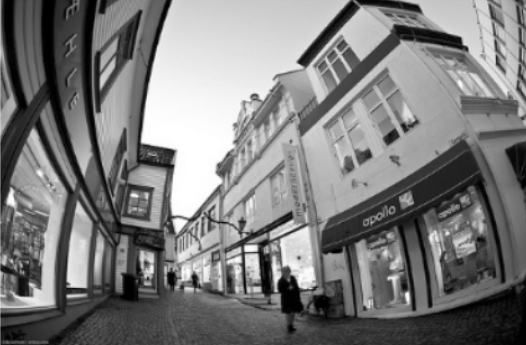
\includegraphics[width=0.5\linewidth]{distortion}
    \caption{Пример фотографии с радиальной дисторсией}
    \label{img:distortion}
    % Source: http://www.cs.ait.ac.th/vgl/faisal/paper/JMIV-Paper.pdf
\end{figure}

Далее будем считать, что при $i>3$ $k_i = 0$. Если параметры $k_1, k_2, k_3$ известны, то построение изображения, преобразование которого совпадает с полученной искаженной фотографией, не вызывает проблем. Необходимо создать изображение $I'$, заполненное нулями, и для каждого пикселя искаженного изображения $I_d$ выполняется следующая операция:
\begin{equation*}
    I'(x(x_d, y_d), y(x_d, y_d)) += I_d(x_d, y_d).
\end{equation*}
Преимущество такого преобразования состоит в том, что несмотря на то, что длины кривых не сохраняются, интегральная яркость вдоль каждой кривой остается той же самой. Но для такой реконструкции требуется уметь находить обратную функцию $f^{-1}(r)$ к \eqref{distortion_eq}.

Предположим, что оригинальная фотография без искажений содержит множество прямых линий и нужно восстановить эту фотографию по искаженной версии. В таком случае можно перебором в некотором пространстве параметров найти параметры, при которых некоторая метрика, описывающая <<прямолинейность>> изображения, достигает максимума. Эта целевая функция вычисляется при помощи быстрого преобразования Хафа.

Качество восстановления изображения с выбранными параметрами оценивается следующим образом:
\begin{enumerate}
\item
    С использованием численных методов находится функция $f^{-1}(r)$. При этом функция $f(r)$ должна быть монотонной на определенном отрезке, в противном случае предложенные параметры не рассматриваются.
\item
    На изображении выделяются границы при помощи оценки градиента яркости.
\item
    Стоится восстановленние изображение, соответствующее оцениваемым параметрам дисторсии.
\item
    Стоится преобразование Хафа для данного изображения. При этом размер матрицы увеличивается вчетверо, поскольку вычисляются суммы по прямым всех ориентаций.
\item
    Из Хаф-образа вычитается этот же образ, сглаженный Гауссовым фильтром; отрицательные значения заменяются на $0$. Полученная матрица обозначается как $H$.
\item
    Вычисляется вектор $F$, содержащий дисперсии значений матрицы $H$ по строкам. Каждый элемент $F_i$ содержит дисперсию значений, соответствующих прямым с одинаковой тангентой $t = t_i$.
\item
    Пусть полученный вектор $F$ имеет $K$ уровней значений, частоты появления которых $P(F_k)$. Тогда в качестве целевой функции используется энтропия $F$:
    \begin{equation*}
        E\left( F \right) =
        -\sum_{k=1}^{K} P(F_k) \log P(F_k)
        \to \min
    \end{equation*}
\end{enumerate}

